\chapter{Cơ sở lý thuyết: Nhận diện biển số xe}
\label{ch:ly_thuyet_alpr}

\section{Phát biểu bài toán ALPR}

\subsection{Định nghĩa bài toán}
Nhận diện biển số xe tự động (Automatic License Plate Recognition - ALPR) là bài toán trích xuất thông tin ký tự từ biển số xe trong ảnh hoặc video một cách tự động. Đây là một bài toán con của nhận dạng ký tự quang học (OCR) được chuyên biệt hóa cho ngữ cảnh giao thông.

\textbf{Phát biểu hình thức:} Cho một ảnh đầu vào $I \in \mathbb{R}^{H \times W \times 3}$ chứa phương tiện giao thông, hệ thống ALPR cần thực hiện:
\begin{enumerate}
    \item \textbf{Plate Detection:} Xác định vùng chứa biển số $R = (x, y, w, h)$ trong ảnh
    \item \textbf{Character Recognition:} Nhận dạng chuỗi ký tự $S = (c_1, c_2, \dots, c_n)$ trên biển số
\end{enumerate}

\subsection{Đặc tả đầu vào/đầu ra}

\begin{table}[!ht]
\centering
\caption{Đặc tả Input/Output của hệ thống ALPR}
\label{tab:alpr_io_spec}
\begin{tabular}{|l|p{10cm}|}
\hline
\textbf{Thành phần} & \textbf{Mô tả chi tiết} \\ \hline
\multicolumn{2}{|c|}{\textbf{ĐẦU VÀO}} \\ \hline
Ảnh/Frame video & Ảnh RGB kích thước $H \times W \times 3$, chứa ít nhất một phương tiện \\ \hline
Độ phân giải tối thiểu & Biển số chiếm ít nhất $50 \times 15$ pixels trong ảnh \\ \hline
Chất lượng & Ảnh không quá mờ (motion blur < 5px), độ sáng đủ \\ \hline
\multicolumn{2}{|c|}{\textbf{ĐẦU RA}} \\ \hline
Bounding box biển số & Tọa độ $(x, y, w, h)$ của vùng biển số trong ảnh \\ \hline
Chuỗi ký tự & Chuỗi 7-9 ký tự (VD: ``30G07784'' hoặc ``29H1234.56'') \\ \hline
Độ tin cậy & Confidence score $\in [0, 1]$ cho mỗi dự đoán \\ \hline
\end{tabular}
\end{table}

\subsection{Ý nghĩa thực tiễn}
Hệ thống ALPR có vai trò quan trọng trong nhiều ứng dụng thực tế tại Việt Nam:

\begin{itemize}
    \item \textbf{Thu phí tự động (ETC):} Giảm thời gian chờ tại trạm thu phí từ 30-60 giây xuống còn 2-3 giây, tăng lưu lượng thông qua 5-10 lần \cite{vtc2024etc}.
    \item \textbf{Quản lý bãi đỗ xe:} Tự động hóa quy trình ra/vào, giảm nhân sự vận hành 70-80\%, tăng năng suất xử lý.
    \item \textbf{Giám sát vi phạm:} Hỗ trợ camera phạt nguội ghi nhận biển số xe vi phạm, tăng tính răn đe và minh bạch.
    \item \textbf{Kiểm soát an ninh:} Phát hiện xe đăng ký trong danh sách cấm/nghi vấn tại các cổng ra vào quan trọng.
    \item \textbf{Thống kê giao thông:} Phân tích lưu lượng xe theo vùng, thời gian, hỗ trợ quy hoạch giao thông.
\end{itemize}

\section{Tổng quan về ALPR}
Hệ thống nhận diện biển số xe tự động (Automatic License Plate Recognition - ALPR) thường bao gồm hai giai đoạn chính:
\begin{enumerate}
    \item \textbf{Plate Detection:} Xác định vị trí biển số trong ảnh
    \item \textbf{Character Recognition (OCR):} Nhận dạng các ký tự trên biển số
\end{enumerate}

\begin{figure}[!htbp]
    \centering
    \begin{tikzpicture}[
        node distance=1cm,
        box/.style={rectangle, draw, rounded corners, minimum width=2.2cm, minimum height=0.9cm, align=center, fill=blue!10, font=\small},
        arrow/.style={->, thick, >=stealth}
    ]
        \node[box] (input) {Ảnh\\đầu vào};
        \node[box, right=of input] (detect) {Plate\\Detection};
        \node[box, right=of detect] (preprocess) {Tiền xử lý\\(CLAHE)};
        \node[box, right=of preprocess] (ocr) {OCR};
        \node[box, right=of ocr] (output) {Biển số};

        \draw[arrow] (input) -- (detect);
        \draw[arrow] (detect) -- (preprocess);
        \draw[arrow] (preprocess) -- (ocr);
        \draw[arrow] (ocr) -- (output);
    \end{tikzpicture}
    \caption{Pipeline tổng quan của hệ thống ALPR}
    \label{fig:alpr_pipeline}
\end{figure}

\section{Biển số xe Việt Nam}

\subsection{Các định dạng biển số}
Biển số xe Việt Nam có các định dạng chính sau:

\begin{table}[!ht]
\centering
\caption{Các định dạng biển số xe Việt Nam}
\label{tab:vn_plate_format}
\begin{tabular}{|c|l|l|}
\hline
\textbf{Loại} & \textbf{Định dạng} & \textbf{Ví dụ} \\ \hline
Xe ô tô (1 dòng) & XX-Y XXXXX & 30G-07784 \\ \hline
Xe ô tô (2 dòng) & XX-Y / XXXXX & 30G / 07784 \\ \hline
Xe máy & XX-YY / XXX.XX & 29-H1 / 234.56 \\ \hline
\end{tabular}
\end{table}

Trong đó:
\begin{itemize}
    \item 2 chữ số đầu: Mã tỉnh/thành phố (VD: 30 = Hà Nội, 29 = Hà Nội cũ, 51 = TP.HCM)
    \item Chữ cái: Ký hiệu seri (A-Z, trừ I, O, Q)
    \item 5 chữ số cuối: Số thứ tự đăng ký
\end{itemize}

\subsection{Thách thức nhận diện biển số Việt Nam}
Việc nhận diện biển số Việt Nam gặp một số thách thức đặc thù, được phân loại thành các nhóm sau:

\subsubsection{Thách thức về dữ liệu}
\begin{itemize}
    \item \textbf{Đa dạng định dạng:} Biển số Việt Nam có nhiều định dạng khác nhau (1 dòng, 2 dòng), kích thước khác nhau giữa xe máy và ô tô, gây khó khăn cho việc chuẩn hóa đầu vào.
    \item \textbf{Dữ liệu không cân bằng:} Trong thực tế, xe máy chiếm tỷ lệ lớn (>70\%) trong dòng giao thông Việt Nam, dẫn đến mất cân bằng lớp khi huấn luyện.
    \item \textbf{Thiếu dữ liệu gán nhãn:} Việc gán nhãn ký tự trên biển số đòi hỏi thời gian và chi phí lớn, trong khi các bộ dữ liệu công khai cho biển số Việt Nam còn hạn chế.
\end{itemize}

\subsubsection{Thách thức về chất lượng ảnh}
\begin{itemize}
    \item \textbf{Độ phân giải thấp:} Camera giám sát thường có độ phân giải thấp, biển số có thể chỉ chiếm vài chục pixel.
    \item \textbf{Motion blur:} Xe di chuyển nhanh gây nhòe ảnh, làm mất nét các ký tự.
    \item \textbf{Biển số bị hư hỏng:} Biển số cũ, bị bẩn, rỉ sét, mờ chữ do thời tiết, hoặc bị che khuất một phần.
    \item \textbf{Điều kiện ánh sáng:} Ánh sáng ban đêm, ngược sáng, phản chiếu từ mặt biển số kim loại gây khó khăn cho nhận dạng.
\end{itemize}

\begin{figure}[!htbp]
    \centering
    \begin{subfigure}[b]{0.3\textwidth}
        \centering
        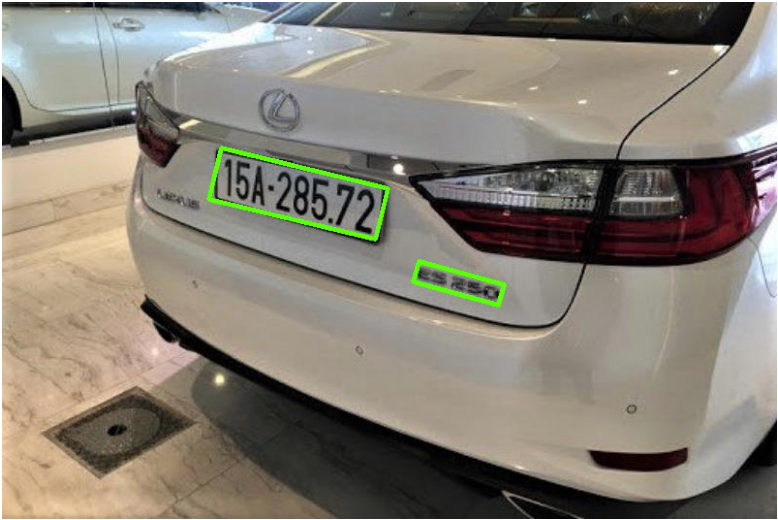
\includegraphics[width=\textwidth]{Figures/plate_perspective.jpg}
        \caption{Biển số nghiêng}
    \end{subfigure}
    \hfill
    \begin{subfigure}[b]{0.3\textwidth}
        \centering
        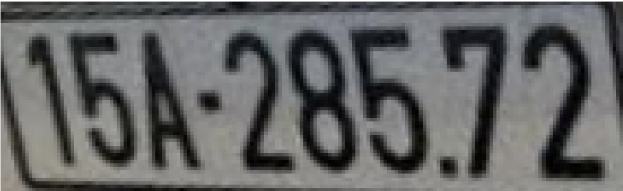
\includegraphics[width=\textwidth]{Figures/plate_rectified.jpg}
        \caption{Biển số rõ}
    \end{subfigure}
    \caption{Ví dụ về thách thức chất lượng ảnh biển số trong thực tế}
    \label{fig:plate_challenges}
\end{figure}

\subsubsection{Thách thức về kỹ thuật}
\begin{itemize}
    \item \textbf{Yêu cầu thời gian thực:} Hệ thống giám sát giao thông cần xử lý 25-30 FPS, đặt ra yêu cầu về tốc độ inference của cả detection và OCR.
    \item \textbf{Font chữ đặc thù:} Font chữ trên biển số Việt Nam có một số điểm khác biệt so với font chuẩn (ví dụ: số 0 và chữ O, số 1 và chữ I).
    \item \textbf{Ký tự tương tự:} Một số cặp ký tự dễ nhầm lẫn: 0/O, 1/I, 8/B, 5/S, đòi hỏi cơ chế hiệu chỉnh hậu xử lý.
    \item \textbf{Biến đổi góc nhìn:} Góc quay camera tạo ra biến dạng phối cảnh (perspective distortion), cần module rectification.
\end{itemize}

\subsubsection{Thách thức về triển khai}
\begin{itemize}
    \item \textbf{Tài nguyên tính toán:} Cần cân bằng giữa độ chính xác và tốc độ để triển khai trên phần cứng phổ thông (không có GPU mạnh).
    \item \textbf{Tích hợp hệ thống:} ALPR cần tích hợp với các module khác (detection, tracking, violation detection) trong một pipeline hoàn chỉnh.
    \item \textbf{Xử lý đa frame:} Một xe có thể xuất hiện trong nhiều frame, cần cơ chế voting/validation để có kết quả ổn định.
\end{itemize}

\section{Các phương pháp OCR hiện có cho ALPR}

Trước khi trình bày chi tiết về PaddleOCR (phương pháp được lựa chọn), phần này tổng hợp và so sánh các công cụ OCR phổ biến có thể ứng dụng cho bài toán ALPR.

\subsection{Tổng quan các công cụ OCR}

\subsubsection{Tesseract OCR}
Tesseract \cite{smith2007overview} là engine OCR mã nguồn mở lâu đời nhất (từ 1985, được Google phát triển từ 2006). Phiên bản 4.0+ sử dụng mạng LSTM cho nhận dạng text.

\textbf{Ưu điểm:}
\begin{itemize}
    \item Miễn phí, mã nguồn mở, cộng đồng hỗ trợ lớn
    \item Hỗ trợ nhiều ngôn ngữ (>100 ngôn ngữ)
    \item Dễ tích hợp qua wrapper (pytesseract)
\end{itemize}

\textbf{Nhược điểm:}
\begin{itemize}
    \item Hiệu năng kém với ảnh nhiễu, mờ, nghiêng
    \item Yêu cầu tiền xử lý ảnh phức tạp (binarization, deskew)
    \item Tốc độ chậm so với các giải pháp deep learning hiện đại
    \item Không có module rectification tích hợp
\end{itemize}

\subsubsection{EasyOCR}
EasyOCR \cite{easyocr2020} là thư viện Python dựa trên PyTorch, sử dụng kiến trúc CRNN + CTC cho nhận dạng văn bản.

\textbf{Ưu điểm:}
\begin{itemize}
    \item API đơn giản, dễ sử dụng
    \item Hỗ trợ 80+ ngôn ngữ
    \item Tích hợp sẵn text detection và recognition
\end{itemize}

\textbf{Nhược điểm:}
\begin{itemize}
    \item Tốc độ inference chậm hơn PaddleOCR
    \item Kích thước model lớn hơn
    \item Khả năng xử lý văn bản nghiêng/cong hạn chế
\end{itemize}

\subsubsection{TrOCR (Microsoft)}
TrOCR \cite{li2021trocr} là mô hình Transformer end-to-end cho OCR, kết hợp Vision Transformer (ViT) encoder và Text Transformer decoder.

\textbf{Ưu điểm:}
\begin{itemize}
    \item Độ chính xác cao trên các benchmark
    \item Kiến trúc Transformer hiện đại
    \item Pre-trained model mạnh
\end{itemize}

\textbf{Nhược điểm:}
\begin{itemize}
    \item Yêu cầu tài nguyên GPU lớn
    \item Tốc độ inference chậm cho real-time applications
    \item Không tối ưu cho triển khai edge devices
\end{itemize}

\subsubsection{PaddleOCR (Baidu)}
PaddleOCR \cite{du2020pp} là bộ công cụ OCR của PaddlePaddle với kiến trúc PP-OCR/PP-OCRv4, sử dụng SVTR backbone.

\textbf{Ưu điểm:}
\begin{itemize}
    \item Cân bằng tốt giữa độ chính xác và tốc độ
    \item Model nhẹ (SVTR\_LCNet chỉ ~12MB)
    \item Tích hợp rectification (STN/TPS) cho văn bản nghiêng
    \item Hỗ trợ nhiều backend (CPU, GPU, TensorRT)
    \item Cộng đồng Trung Quốc lớn, nhiều tài liệu tiếng Việt
\end{itemize}

\textbf{Nhược điểm:}
\begin{itemize}
    \item Phụ thuộc PaddlePaddle framework
    \item Một số lỗi với ký tự đặc biệt
\end{itemize}

\subsection{Bảng so sánh các phương pháp}

\begin{table}[!ht]
\centering
\caption{So sánh các công cụ OCR cho bài toán ALPR}
\label{tab:ocr_comparison}
\begin{tabular}{|l|c|c|c|c|}
\hline
\textbf{Tiêu chí} & \textbf{Tesseract} & \textbf{EasyOCR} & \textbf{TrOCR} & \textbf{PaddleOCR} \\ \hline
Độ chính xác & Trung bình & Khá & Cao & Cao \\ \hline
Tốc độ inference & Chậm & Trung bình & Chậm & Nhanh \\ \hline
Kích thước model & Nhỏ & Lớn & Rất lớn & Nhỏ \\ \hline
Xử lý text nghiêng & Kém & Trung bình & Khá & Tốt (TPS) \\ \hline
Real-time capable & Không & Hạn chế & Không & Có \\ \hline
Dễ tích hợp & Trung bình & Tốt & Trung bình & Tốt \\ \hline
\end{tabular}
\end{table}

\subsection{Lý do lựa chọn PaddleOCR}
Sau khi phân tích các phương pháp, chúng tôi lựa chọn \textbf{PaddleOCR} cho dự án với các lý do sau:

\begin{enumerate}
    \item \textbf{Cân bằng accuracy-speed:} PaddleOCR cung cấp sự cân bằng tốt nhất giữa độ chính xác và tốc độ, quan trọng cho ứng dụng real-time.
    
    \item \textbf{Xử lý biển số nghiêng:} Tích hợp sẵn module rectification (STN/TPS) giúp xử lý biển số bị biến dạng do góc camera mà không cần tiền xử lý phức tạp.
    
    \item \textbf{Model nhẹ:} SVTR\_LCNet chỉ ~12MB, phù hợp triển khai trên phần cứng phổ thông và edge devices.
    
    \item \textbf{Tương thích tốt:} Hỗ trợ nhiều backend (CPU, GPU, TensorRT), dễ dàng tích hợp vào pipeline Python hiện có.
    
    \item \textbf{Cập nhật liên tục:} Baidu liên tục cải tiến PaddleOCR với các phiên bản PP-OCRv2, v3, v4.
\end{enumerate}

\section{PaddleOCR - Nhận dạng ký tự}

\subsection{Giới thiệu PaddleOCR}
PaddleOCR là một bộ công cụ OCR mã nguồn mở được phát triển bởi PaddlePaddle (Baidu). Trong dự án này, chúng tôi sử dụng \textbf{PaddleOCR phiên bản 2.7.x} (tương ứng với PP-OCRv4). PaddleOCR hỗ trợ nhận dạng văn bản đa ngôn ngữ (hơn 80 ngôn ngữ) với kiến trúc linh hoạt, phù hợp cho nhiều bài toán OCR. 

Trong đề tài này, chúng tôi sử dụng PaddleOCR với tham số \texttt{use\_textline\_orientation=True} để tự động phát hiện và xoay văn bản nghiêng, kết hợp với \texttt{lang='en'} cho bộ ký tự Latin (phù hợp với biển số Việt Nam).

\subsection{Pipeline nhận dạng văn bản trong PaddleOCR}

PaddleOCR sử dụng một pipeline hoàn chỉnh để nhận dạng văn bản, bao gồm các bước chính:

\begin{figure}[!htbp]
    \centering
    \begin{tikzpicture}[
        node distance=0.8cm,
        box/.style={rectangle, draw, rounded corners, minimum width=2cm, minimum height=0.8cm, align=center, fill=blue!10, font=\footnotesize},
        arrow/.style={->, thick, >=stealth}
    ]
        \node[box] (input) {Ảnh biển số\\(nghiêng/cong)};
        \node[box, right=of input] (rect) {Rectification\\(STN/TPS)};
        \node[box, right=of rect] (backbone) {Feature\\Extraction};
        \node[box, right=of backbone] (seq) {Sequence\\Modeling};
        \node[box, right=of seq] (ctc) {CTC\\Decoder};
        \node[box, right=of ctc] (output) {``15A-285.72''};

        \draw[arrow] (input) -- (rect);
        \draw[arrow] (rect) -- (backbone);
        \draw[arrow] (backbone) -- (seq);
        \draw[arrow] (seq) -- (ctc);
        \draw[arrow] (ctc) -- (output);
    \end{tikzpicture}
    \caption{Pipeline nhận dạng văn bản trong PaddleOCR}
    \label{fig:paddleocr_pipeline}
\end{figure}

%============================================================
% SUBSECTION: RECTIFICATION
%============================================================
\subsection{Rectification - Nắn thẳng biển số}

Biển số xe trong thực tế thường bị nghiêng, xoay hoặc biến dạng do góc chụp camera. Để giảm ảnh hưởng của góc chụp và biến dạng, PaddleOCR sử dụng module \textbf{Rectification} để tự động nắn thẳng ảnh văn bản trước khi đưa vào mô hình nhận dạng.

\begin{figure}[!htbp]
    \centering
    \begin{subfigure}[b]{0.45\textwidth}
        \centering
        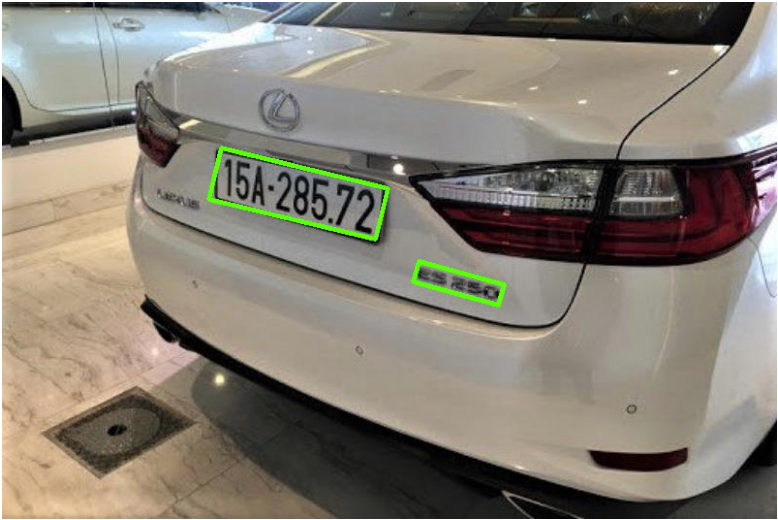
\includegraphics[width=\textwidth]{Figures/plate_perspective.jpg}
        \caption{Biển số bị nghiêng do góc camera}
        \label{fig:plate_perspective}
    \end{subfigure}
    \hfill
    \begin{subfigure}[b]{0.45\textwidth}
        \centering
        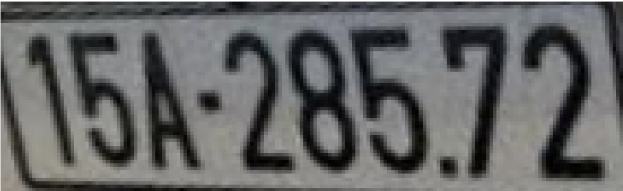
\includegraphics[width=\textwidth]{Figures/plate_rectified.jpg}
        \caption{Biển số sau khi nắn thẳng}
        \label{fig:plate_rectified}
    \end{subfigure}
    \caption{Minh họa quá trình Rectification biển số xe}
    \label{fig:rectification_example}
\end{figure}

\subsubsection{Spatial Transformer Network (STN)}
STN (Spatial Transformer Network) \cite{jaderberg2015spatial} là một module học sâu cho phép mạng neural tự động học cách biến đổi không gian của ảnh đầu vào. STN bao gồm 3 thành phần:

\begin{enumerate}
    \item \textbf{Localization Network:} Mạng CNN nhỏ học các tham số biến đổi $\theta$ từ ảnh đầu vào
    \item \textbf{Grid Generator:} Tạo lưới tọa độ cho ảnh output dựa trên $\theta$
    \item \textbf{Sampler:} Lấy mẫu pixel từ ảnh gốc theo lưới tọa độ đã tính
\end{enumerate}

\begin{figure}[!htbp]
    \centering
    \begin{tikzpicture}[
        node distance=0.6cm,
        box/.style={rectangle, draw, rounded corners, minimum width=1.8cm, minimum height=0.7cm, align=center, fill=orange!15, font=\footnotesize},
        arrow/.style={->, thick, >=stealth}
    ]
        \node[box] (input) {Ảnh nghiêng\\$I$};
        \node[box, right=of input] (loc) {Localization\\Network};
        \node[box, right=of loc] (theta) {Tham số\\$\theta$};
        \node[box, right=of theta] (grid) {Grid\\Generator};
        \node[box, right=of grid] (sample) {Sampler};
        \node[box, right=of sample] (output) {Ảnh thẳng\\$I'$};

        \draw[arrow] (input) -- (loc);
        \draw[arrow] (loc) -- (theta);
        \draw[arrow] (theta) -- (grid);
        \draw[arrow] (grid) -- (sample);
        \draw[arrow] (sample) -- (output);
        \draw[arrow, dashed] (input) to[bend right=30] (sample);
    \end{tikzpicture}
    \caption{Kiến trúc Spatial Transformer Network}
    \label{fig:stn_arch}
\end{figure}

\textbf{Phép biến đổi Affine:}
Với phép biến đổi affine 2D, ma trận tham số $\theta$ có dạng:
\begin{equation}
    \theta = \begin{bmatrix}
        \theta_{11} & \theta_{12} & \theta_{13} \\
        \theta_{21} & \theta_{22} & \theta_{23}
    \end{bmatrix}
\end{equation}

Tọa độ điểm $(x_i^s, y_i^s)$ trong ảnh nguồn được tính từ tọa độ $(x_i^t, y_i^t)$ trong ảnh đích:
\begin{equation}
    \begin{pmatrix} x_i^s \\ y_i^s \end{pmatrix} = \begin{bmatrix}
        \theta_{11} & \theta_{12} & \theta_{13} \\
        \theta_{21} & \theta_{22} & \theta_{23}
    \end{bmatrix} \begin{pmatrix} x_i^t \\ y_i^t \\ 1 \end{pmatrix}
\end{equation}

Phép biến đổi affine có thể biểu diễn: xoay (rotation), co giãn (scale), dịch chuyển (translation), và nghiêng (shear).

\subsubsection{Thin-Plate Spline (TPS) Transformation}
Đối với văn bản bị uốn cong (curved text), phép biến đổi affine không đủ linh hoạt. PaddleOCR sử dụng \textbf{TPS (Thin-Plate Spline)} \cite{shi2016robust} để xử lý các biến dạng phi tuyến tính phức tạp hơn.

TPS sử dụng một tập các điểm điều khiển (control points) $\{(x_k, y_k)\}_{k=1}^{K}$ để định nghĩa phép biến đổi. Công thức TPS:
\begin{equation}
    f(x, y) = a_0 + a_x x + a_y y + \sum_{k=1}^{K} w_k \cdot U(||(x, y) - (x_k, y_k)||)
\end{equation}

Trong đó:
\begin{itemize}
    \item $a_0, a_x, a_y$: Các tham số affine
    \item $w_k$: Trọng số của điểm điều khiển thứ $k$
    \item $U(r) = r^2 \log(r)$: Hàm cơ sở radial basis function (RBF)
    \item $K$: Số điểm điều khiển (thường $K = 20$ trong PaddleOCR)
\end{itemize}

\begin{figure}[!htbp]
    \centering
    \begin{tikzpicture}[scale=0.9]
        % Input curved text
        \draw[thick, blue] (0,0) .. controls (0.5,0.8) and (1.5,0.8) .. (2,0) 
                           .. controls (2.5,-0.3) and (3.5,-0.3) .. (4,0);
        \node at (2,-0.8) {Văn bản cong (input)};
        
        % Arrow
        \draw[->, very thick] (4.5,0) -- (5.5,0);
        \node at (5,0.4) {TPS};
        
        % Output straight text
        \draw[thick, green!60!black] (6,0) -- (10,0);
        \node at (8,-0.8) {Văn bản thẳng (output)};
        
        % Control points on curved
        \foreach \x in {0,0.8,1.6,2.4,3.2,4}
            \fill[red] (\x,{0.4*sin(\x*90)}) circle (2pt);
        
        % Control points on straight
        \foreach \x in {6,6.8,7.6,8.4,9.2,10}
            \fill[red] (\x,0) circle (2pt);
    \end{tikzpicture}
    \caption{TPS transformation nắn thẳng văn bản cong}
    \label{fig:tps_transform}
\end{figure}

\subsubsection{Ứng dụng trong PaddleOCR}
Khi khởi tạo PaddleOCR với \texttt{use\_textline\_orientation=True}:
\begin{itemize}
    \item Mô hình tự động phát hiện hướng của văn bản
    \item Áp dụng phép xoay để đưa văn bản về hướng ngang
    \item Với văn bản nghiêng/cong, module TPS được kích hoạt để nắn thẳng
    \item Ảnh đã được rectified được đưa vào mô hình nhận dạng chính
\end{itemize}

%============================================================
% SUBSECTION: SVTR ARCHITECTURE
%============================================================
\subsection{Kiến trúc SVTR - Scene Text Recognition}

Từ phiên bản PP-OCRv3, PaddleOCR đã chuyển từ kiến trúc CRNN truyền thống sang \textbf{SVTR} (Single Visual model for Scene Text Recognition) \cite{du2022svtr}. SVTR là một kiến trúc hiệu quả hơn, sử dụng hoàn toàn cơ chế attention thay vì RNN.

\begin{figure}[!htbp]
    \centering
    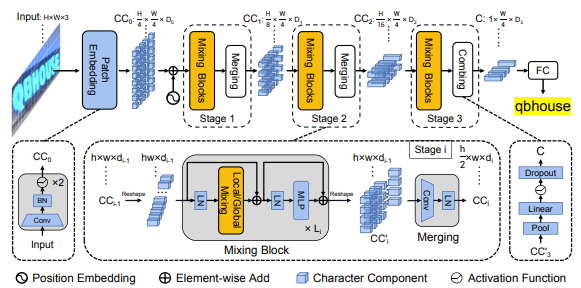
\includegraphics[width=0.95\textwidth]{Figures/svtr_architecture.png}
    \caption{Kiến trúc tổng quan của SVTR (nguồn: Du et al., 2022)}
    \label{fig:svtr_architecture}
\end{figure}

\subsubsection{Ý tưởng chính của SVTR}
SVTR xử lý ảnh văn bản bằng cách:
\begin{enumerate}
    \item \textbf{Patch Embedding:} Chia ảnh thành các patch nhỏ (character components)
    \item \textbf{Hierarchical Mixing:} Trộn thông tin qua nhiều tầng với local và global attention
    \item \textbf{Linear Prediction:} Dự đoán ký tự trực tiếp từ feature cuối
\end{enumerate}

\begin{figure}[!htbp]
    \centering
    \begin{tikzpicture}[
        node distance=0.5cm,
        patch/.style={rectangle, draw, minimum width=0.4cm, minimum height=0.6cm, fill=yellow!30},
        box/.style={rectangle, draw, rounded corners, minimum width=2cm, minimum height=0.7cm, align=center, fill=green!15, font=\footnotesize},
        arrow/.style={->, thick, >=stealth}
    ]
        % Input image with patches
        \node[box, minimum width=3cm] (input) {Ảnh biển số\\$H \times W \times 3$};
        
        % Patch embedding
        \node[box, right=0.8cm of input] (patch) {Patch Embedding\\$\frac{H}{4} \times \frac{W}{4} \times D$};
        
        % Mixing stages
        \node[box, right=0.8cm of patch, fill=blue!15] (local) {Local\\Mixing};
        \node[box, right=0.5cm of local, fill=blue!15] (global) {Global\\Mixing};
        \node[box, right=0.5cm of global, fill=blue!15] (merge) {Merging\\Stage};
        
        % Output
        \node[box, right=0.8cm of merge, fill=red!15] (pred) {CTC/Attn\\Decoder};
        \node[box, right=0.5cm of pred] (output) {``15A-285.72''};

        \draw[arrow] (input) -- (patch);
        \draw[arrow] (patch) -- (local);
        \draw[arrow] (local) -- (global);
        \draw[arrow] (global) -- (merge);
        \draw[arrow] (merge) -- (pred);
        \draw[arrow] (pred) -- (output);
    \end{tikzpicture}
    \caption{Kiến trúc SVTR trong PaddleOCR}
    \label{fig:svtr_arch}
\end{figure}

\subsubsection{Cơ chế cắt Patch và trích xuất đặc trưng}

SVTR xử lý ảnh văn bản giống như Vision Transformer (ViT), nhưng được tối ưu cho văn bản:

\textbf{Bước 1 - Patch Embedding:}
\begin{itemize}
    \item Ảnh đầu vào kích thước $H \times W \times 3$ được chia thành các patch kích thước $4 \times 4$
    \item Mỗi patch được flatten và chiếu lên không gian $D$ chiều
    \item Kết quả: chuỗi $T = \frac{H}{4} \times \frac{W}{4}$ token, mỗi token là vector $D$ chiều
\end{itemize}

\textbf{Bước 2 - Local Mixing (Intra-character):}
\begin{itemize}
    \item Học các đặc trưng \textbf{bên trong} từng ký tự (nét, đường cong, góc)
    \item Sử dụng window-based self-attention với window size nhỏ
    \item Cho phép các patch lân cận trao đổi thông tin
\end{itemize}

\textbf{Bước 3 - Global Mixing (Inter-character):}
\begin{itemize}
    \item Học mối quan hệ \textbf{giữa các ký tự} (ngữ cảnh)
    \item Sử dụng global self-attention trên toàn bộ chuỗi
    \item Giúp phân biệt các ký tự giống nhau dựa trên ngữ cảnh
\end{itemize}

\begin{figure}[!htbp]
    \centering
    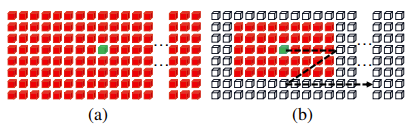
\includegraphics[width=0.85\textwidth]{Figures/svtr_local_global_mixing.png}
    \caption{So sánh Local Mixing và Global Mixing trong SVTR}
    \label{fig:svtr_mixing}
\end{figure}

\textbf{Bước 4 - Height Merging:}
\begin{itemize}
    \item Gộp các token theo chiều cao để tạo chuỗi 1D
    \item Giảm từ $\frac{H}{4} \times \frac{W}{4}$ thành $1 \times \frac{W}{4}$ token
    \item Mỗi token đại diện cho một ``lát cắt'' dọc của ảnh
\end{itemize}

\begin{figure}[!htbp]
    \centering
    \begin{tikzpicture}
        % License plate image với hình thật
        \node[inner sep=0] (plate) at (0,0) {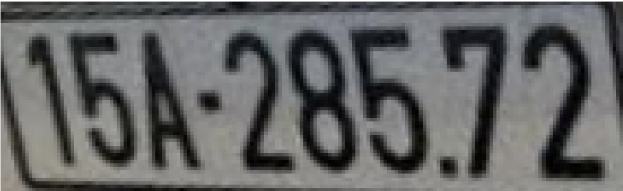
\includegraphics[width=8cm]{Figures/plate_rectified.jpg}};
        
        % Vertical slices - vẽ các đường cắt dọc
        \foreach \x in {-3.5,-2.5,...,3.5} {
            \draw[dashed, blue!70, thick] (\x,-0.6) -- (\x,0.6);
        }
        
        % Feature vectors below
        \foreach \x in {-3.5,-2.5,...,3.5} {
            \draw[->, thick, red!70] (\x,-0.7) -- (\x,-1.1);
        }
        
        % Labels
        \node at (0,-1.5) {Ảnh biển số được chia thành các ``lát cắt'' dọc};
        \node at (0,-2.0) {$\downarrow$ mỗi lát $\rightarrow$ vector đặc trưng $D$ chiều};
    \end{tikzpicture}
    \caption{Minh họa cắt ảnh thành các lát dọc trong SVTR}
    \label{fig:svtr_slices}
\end{figure}

\subsubsection{So sánh SVTR và CRNN}

\begin{table}[!ht]
\centering
\caption{So sánh kiến trúc SVTR và CRNN}
\label{tab:svtr_vs_crnn}
\begin{tabular}{|l|p{5cm}|p{5cm}|}
\hline
\textbf{Tiêu chí} & \textbf{CRNN} & \textbf{SVTR} \\ \hline
Trích xuất đặc trưng & CNN (ResNet, MobileNet) & Patch Embedding + Transformer \\ \hline
Mô hình hóa chuỗi & Bidirectional LSTM & Self-Attention (Local + Global) \\ \hline
Tính toán & Tuần tự & Song song \\ \hline
Ngữ cảnh & Hạn chế bởi hidden size LSTM & Toàn cục qua attention \\ \hline
\end{tabular}
\end{table}

%============================================================
% SUBSECTION: CRNN ARCHITECTURE (Legacy)
%============================================================
\subsection{Kiến trúc CRNN (Legacy)}

Mặc dù SVTR là mặc định trong các phiên bản mới, PaddleOCR vẫn hỗ trợ kiến trúc CRNN truyền thống. CRNN (Convolutional Recurrent Neural Network) bao gồm:

\begin{enumerate}
    \item \textbf{CNN Backbone:} Trích xuất đặc trưng không gian từ ảnh đầu vào. Backbone thường sử dụng là MobileNet hoặc ResNet biến thể.
    \item \textbf{Sequence Modeling (LSTM):} Mô hình hóa quan hệ tuần tự giữa các ký tự. Sử dụng Bidirectional LSTM để capture thông tin từ cả hai hướng.
    \item \textbf{CTC Decoder:} Giải mã chuỗi ký tự cuối cùng từ output của LSTM.
\end{enumerate}

\begin{figure}[!htbp]
    \centering
    \begin{tikzpicture}[
        node distance=1cm,
        box/.style={rectangle, draw, rounded corners, minimum width=2.2cm, minimum height=0.9cm, align=center, fill=green!10, font=\small},
        arrow/.style={->, thick, >=stealth}
    ]
        \node[box] (input) {Ảnh biển số\\$H \times W$};
        \node[box, right=of input] (cnn) {CNN\\Backbone};
        \node[box, right=of cnn] (lstm) {Bi-LSTM\\$T \times D$};
        \node[box, right=of lstm] (ctc) {CTC\\Decoder};
        \node[box, right=of ctc] (output) {15A-285.72};

        \draw[arrow] (input) -- (cnn);
        \draw[arrow] (cnn) -- (lstm);
        \draw[arrow] (lstm) -- (ctc);
        \draw[arrow] (ctc) -- (output);
    \end{tikzpicture}
    \caption{Kiến trúc CRNN cho OCR trong PaddleOCR}
    \label{fig:crnn_arch}
\end{figure}

%============================================================
% SUBSECTION: CTC DECODER
%============================================================
\subsection{CTC Decoder - Giải mã chuỗi ký tự}

CTC (Connectionist Temporal Classification) là phương pháp giải mã cho phép huấn luyện mà không cần alignment giữa input và output. Đây là đặc điểm quan trọng vì ta không biết chính xác vị trí của từng ký tự trên ảnh.

\subsubsection{Nguyên lý hoạt động}
Sau khi đi qua backbone (SVTR hoặc CRNN), mỗi ``lát cắt'' dọc của ảnh được biểu diễn bằng một vector xác suất trên tập ký tự (bao gồm cả ký tự đặc biệt ``blank'' $\epsilon$).

\textbf{Ví dụ:} Với ảnh biển số ``15A'', output của mô hình có thể là:
\begin{center}
\begin{tabular}{|c|c|c|c|c|c|c|c|}
\hline
Lát & 1 & 2 & 3 & 4 & 5 & 6 & 7 \\ \hline
Output & 1 & 1 & $\epsilon$ & 5 & $\epsilon$ & A & A \\ \hline
\end{tabular}
\end{center}

Sau khi áp dụng CTC collapse (loại bỏ lặp và blank): ``11-5-AA'' $\rightarrow$ ``15A''

\subsubsection{Công thức xác suất CTC}
Xác suất của một chuỗi output $\mathbf{l}$ được tính:
\begin{equation}
    P(\mathbf{l} | \mathbf{x}) = \sum_{\pi \in \mathcal{B}^{-1}(\mathbf{l})} P(\pi | \mathbf{x})
\end{equation}

Trong đó:
\begin{itemize}
    \item $\mathbf{x}$: Chuỗi feature vectors (từ các lát cắt)
    \item $\mathbf{l}$: Chuỗi ký tự mục tiêu (VD: ``15A-285.72'')
    \item $\pi$: Một alignment path (VD: ``1-5-A---2-8-5-...'')
    \item $\mathcal{B}^{-1}(\mathbf{l})$: Tập tất cả các path có thể tạo ra $\mathbf{l}$ sau khi loại bỏ ký tự blank và ký tự lặp
\end{itemize}

\textbf{Ví dụ:} Với chuỗi mục tiêu ``AB'', các path hợp lệ có thể là:
\begin{itemize}
    \item ``A-A-B-B'' $\rightarrow$ ``AB'' (loại bỏ lặp)
    \item ``A--B-'' $\rightarrow$ ``AB'' (loại bỏ blank `-')
    \item ``-A-B-'' $\rightarrow$ ``AB''
\end{itemize}

\subsubsection{Greedy Decoding và Beam Search}
Trong inference, CTC decoder sử dụng:

\textbf{Greedy Decoding (mặc định):}
\begin{itemize}
    \item Tại mỗi timestep, chọn ký tự có xác suất cao nhất
    \item Sau đó áp dụng collapse rule
    \item Đơn giản, không duy trì nhiều giả thuyết
\end{itemize}

\textbf{Beam Search:}
\begin{itemize}
    \item Duy trì $k$ hypotheses tốt nhất tại mỗi bước
    \item Cộng dồn log-probability của các ký tự
    \item Mở rộng không gian giả thuyết trong quá trình giải mã
\end{itemize}

\subsubsection{CTC Loss}
CTC Loss được tính bằng negative log-likelihood:
\begin{equation}
    \mathcal{L}_{CTC} = -\log P(\mathbf{l} | \mathbf{x})
\end{equation}

Để tính toán hiệu quả, sử dụng thuật toán forward-backward tương tự HMM.

\section{Tiền xử lý ảnh biển số}

Chất lượng ảnh biển số ảnh hưởng trực tiếp đến khả năng nhận dạng của OCR. Chúng tôi áp dụng các kỹ thuật tiền xử lý sau:

\subsection{CLAHE - Cân bằng histogram thích ứng}
CLAHE (Contrast Limited Adaptive Histogram Equalization) là kỹ thuật cải thiện độ tương phản ảnh, đặc biệt hiệu quả cho ảnh có độ sáng không đều.

\subsubsection{Nguyên lý hoạt động}
\begin{enumerate}
    \item \textbf{Chia tile:} Chia ảnh thành các tile nhỏ (VD: 8×8 pixels)
    \item \textbf{Histogram Equalization cục bộ:} Thực hiện histogram equalization trên từng tile
    \item \textbf{Clip Limit:} Giới hạn độ tương phản (clip limit) để tránh khuếch đại noise. Nếu histogram bin vượt quá clip limit, phần dư sẽ được phân bố lại đều cho các bin khác.
    \item \textbf{Bilinear Interpolation:} Nội suy bilinear để ghép các tile lại một cách mượt mà, tránh hiện tượng blocking artifact.
\end{enumerate}

\subsubsection{Công thức toán học}
Công thức histogram equalization cho một pixel:
\begin{equation}
    s_k = (L-1) \cdot \sum_{j=0}^{k} p_r(r_j) = (L-1) \cdot \text{CDF}(r_k)
\end{equation}

Trong đó:
\begin{itemize}
    \item $s_k$: Mức xám mới của pixel
    \item $L$: Số mức xám (256 cho ảnh 8-bit)
    \item $p_r(r_j)$: Xác suất xuất hiện của mức xám $r_j$
    \item CDF: Cumulative Distribution Function của histogram
\end{itemize}

\textbf{Clip Limit trong CLAHE:}
\begin{equation}
    \beta = \frac{M \times N}{L} \times \text{clipLimit}
\end{equation}
Trong đó $M \times N$ là kích thước tile và clipLimit là tham số (thường từ 2.0 đến 4.0).

\subsection{Sharpening - Làm sắc nét}
Bộ lọc làm sắc nét giúp tăng cường các cạnh của ký tự, làm cho chúng rõ ràng hơn trước khi đưa vào OCR.

\subsubsection{Kernel Sharpening}
Chúng tôi sử dụng kernel convolution để làm sắc nét:
\begin{equation}
    K_{sharpen} = \begin{bmatrix}
        0 & -1 & 0 \\
        -1 & 5 & -1 \\
        0 & -1 & 0
    \end{bmatrix}
\end{equation}

\subsubsection{Nguyên lý}
Kernel này hoạt động bằng cách:
\begin{itemize}
    \item Nhân pixel trung tâm với hệ số lớn (5)
    \item Trừ đi trung bình của 4 pixel lân cận
    \item Kết quả: tăng cường sự khác biệt giữa pixel và các pixel xung quanh $\rightarrow$ cạnh sắc nét hơn
\end{itemize}

Công thức tính pixel mới:
\begin{equation}
    I'(x,y) = 5 \cdot I(x,y) - [I(x-1,y) + I(x+1,y) + I(x,y-1) + I(x,y+1)]
\end{equation}

\subsection{Quy trình tiền xử lý hoàn chỉnh}
\begin{enumerate}
    \item \textbf{Crop ảnh biển số:} Từ đầu ra detection của YOLOv8
    \item \textbf{Chuyển Grayscale:} Để áp dụng CLAHE
    \item \textbf{Áp dụng CLAHE:} Với \texttt{clipLimit=2.0}, \texttt{tileGridSize=(8,8)}
    \item \textbf{Chuyển về RGB:} Để đưa vào PaddleOCR
    \item \textbf{Sharpening (tùy chọn):} Áp dụng nếu ảnh còn mờ
\end{enumerate}

\section{So sánh các phiên bản YOLOv8}

Trong đề tài này, chúng tôi sử dụng \textbf{YOLOv8n} (nano) cho cả phát hiện phương tiện và phát hiện biển số vì phù hợp với ràng buộc triển khai và tài nguyên.

\begin{table}[!ht]
\centering
\caption{So sánh các phiên bản YOLOv8}
\label{tab:yolov8_versions}
\begin{tabular}{|c|c|c|}
\hline
\textbf{Model} & \textbf{Params (M)} & \textbf{FLOPs (G)} \\ \hline
YOLOv8n & 3.2 & 8.7 \\ \hline
YOLOv8s & 11.2 & 28.6 \\ \hline
YOLOv8m & 25.9 & 78.9 \\ \hline
YOLOv8l & 43.7 & 165.2 \\ \hline
YOLOv8x & 68.2 & 257.8 \\ \hline
\end{tabular}
\end{table}

\textbf{Lý do chọn YOLOv8n:}
\begin{itemize}
    \item Số lượng tham số nhỏ (3.2M) $\rightarrow$ phù hợp triển khai trên phần cứng phổ thông
    \item FLOPs thấp (8.7G) $\rightarrow$ giảm chi phí tính toán
    \item Phù hợp cho bài toán phát hiện biển số một lớp và tích hợp trong pipeline tổng thể
\end{itemize}

\section{Cơ chế Validation \& Retry}

\subsection{Vấn đề với OCR đơn frame}
OCR có thể cho chuỗi đầu ra khác nhau giữa các frame do:
\begin{itemize}
    \item Biển số bị rung, blur khi xe di chuyển
    \item Ánh sáng thay đổi (phản chiếu, bóng)
    \item Góc nhìn thay đổi khi xe tiến lại gần camera
    \item Nhiễu từ mô hình OCR
\end{itemize}

\subsection{Giải pháp: Format Validation}
Thay vì lưu trữ nhiều chuỗi đầu ra và voting, chúng tôi sử dụng phương pháp validate format biển số Việt Nam:

\begin{algorithm}[!ht]
\SetAlgoLined
\KwIn{$ocr\_text$: Chuỗi OCR, $vehicle\_class$: Loại xe}
\KwOut{$(is\_valid, cleaned\_plate)$: Trạng thái hợp lệ và chuỗi đã làm sạch}

$cleaned \leftarrow$ RemoveSpaces($ocr\_text$)\;
\eIf{$vehicle\_class \in \{motorbike, bicycle\}$}{
    $pattern \leftarrow$ ``\textasciicircum{}[0-9]\{2\}[A-Z][A-Z0-9][0-9]\{4,5\}\$''\;
    $min\_len \leftarrow 8$, $max\_len \leftarrow 9$\;
}{
    $pattern \leftarrow$ ``\textasciicircum{}[0-9]\{2\}[A-Z][0-9]\{4,5\}\$''\;
    $min\_len \leftarrow 7$, $max\_len \leftarrow 8$\;
}
\If{$min\_len \leq \text{len}(cleaned) \leq max\_len$ \textbf{AND} Match($pattern$, $cleaned$)}{
    \Return $(True, cleaned)$\;
}
\Return $(False, cleaned)$\;
\caption{Thuật toán Validation biển số Việt Nam}
\label{alg:validation}
\end{algorithm}

\subsection{Retry Mechanism}
Khi chuỗi OCR không đúng format, hệ thống sẽ retry ở frame tiếp theo:
\begin{itemize}
    \item Chỉ lưu chuỗi \textbf{đã validate} (đúng format)
    \item Nếu OCR sai format hoặc không đọc được $\rightarrow$ không lưu, thử lại frame sau
    \item Khi đã có chuỗi hợp lệ $\rightarrow$ không xử lý OCR nữa (tiết kiệm tài nguyên)
\end{itemize}

\begin{equation}
    \text{ShouldRunOCR}(track\_id) = \begin{cases}
        \text{True} & \text{nếu chưa có chuỗi valid} \\
        \text{False} & \text{nếu đã có chuỗi valid}
    \end{cases}
\end{equation}

\section{Character Correction cho biển số Việt Nam}

\subsection{Các lỗi phổ biến của OCR}
Do một số ký tự có hình dáng tương tự, PaddleOCR có thể nhầm lẫn:

\begin{table}[!ht]
\centering
\caption{Bảng hiệu chỉnh ký tự phổ biến}
\label{tab:char_correction}
\begin{tabular}{|c|c|l|}
\hline
\textbf{Sai} & \textbf{Đúng} & \textbf{Điều kiện} \\ \hline
0 (số không) & O (chữ O) & Vị trí chữ cái (index 2) \\ \hline
O (chữ O) & 0 (số không) & Vị trí chữ số \\ \hline
1 (số một) & I (chữ I) & Vị trí chữ cái \\ \hline
8 (số tám) & B (chữ B) & Vị trí chữ cái \\ \hline
5 (số năm) & S (chữ S) & Vị trí chữ cái \\ \hline
\end{tabular}
\end{table}

\subsection{Logic hiệu chỉnh dựa trên định dạng}
Dựa trên cấu trúc biển số Việt Nam (ví dụ: 30G-07784):
\begin{itemize}
    \item \textbf{Vị trí 0-1:} Bắt buộc là chữ số (mã tỉnh)
    \item \textbf{Vị trí 2:} Bắt buộc là chữ cái (seri)
    \item \textbf{Vị trí 3-7:} Bắt buộc là chữ số (số thứ tự)
\end{itemize}

Thuật toán hiệu chỉnh:
\begin{enumerate}
    \item Kiểm tra độ dài chuỗi OCR
    \item Tại mỗi vị trí, kiểm tra xem ký tự có đúng loại (chữ/số) không
    \item Nếu sai loại, tra bảng mapping để sửa
\end{enumerate}

\section{Hai phương pháp triển khai ALPR}

Trong hệ thống của chúng tôi, có hai cách tiếp cận để thực hiện nhận diện biển số xe:

\subsection{Phương pháp 1: Two-Stage ALPR (Hai giai đoạn)}

Đây là phương pháp truyền thống, chia quá trình thành hai bước độc lập:

\subsubsection{Kiến trúc}
\begin{enumerate}
    \item \textbf{Giai đoạn 1 - Phát hiện phương tiện:} Sử dụng YOLOv8n (5 lớp) để phát hiện các loại xe (xe máy, xe đạp, ô tô, xe buýt, xe tải)
    \item \textbf{Giai đoạn 2 - Phát hiện biển số:} Crop vùng xe từ giai đoạn 1, chạy qua YOLOv8n chuyên biệt (1 lớp: license\_plate) để phát hiện biển số
    \item \textbf{Giai đoạn 3 - OCR:} Crop vùng biển số, áp dụng tiền xử lý (CLAHE, sharpening), sau đó sử dụng PaddleOCR để nhận dạng ký tự
\end{enumerate}

\subsubsection{Ưu điểm}
\begin{itemize}
    \item \textbf{Mô hình chuyên biệt:} Tách riêng nhiệm vụ phát hiện biển số để tập trung đặc trưng mục tiêu
    \item \textbf{Tập trung đặc trưng:} Chỉ xử lý một nhiệm vụ (plate detection) nên dễ tối ưu dữ liệu và huấn luyện
    \item \textbf{Linh hoạt:} Có thể thay thế từng module độc lập (ví dụ: thay YOLOv8 bằng Faster R-CNN cho plate detection)
\end{itemize}

\subsubsection{Nhược điểm}
\begin{itemize}
    \item \textbf{Nhiều lần suy luận:} Cần 2 lần inference qua YOLO (vehicle detection + plate detection)
    \item \textbf{Nhiều mô hình:} Phải load 2 mô hình vào GPU/RAM
    \item \textbf{Phức tạp:} Logic phải quản lý 2 models, crop vùng xe, rồi mới detect plate
\end{itemize}

\subsection{Phương pháp 2: One-Stage Semi-supervised (Một giai đoạn)}

Phương pháp này tích hợp việc phát hiện phương tiện và biển số vào một mô hình duy nhất.

\subsubsection{Kiến trúc}
\begin{enumerate}
    \item \textbf{Giai đoạn 1 - Phát hiện đa lớp:} Sử dụng YOLOv8n (6 lớp) để phát hiện đồng thời cả xe và biển số trong một lần forward pass
    \item \textbf{Giai đoạn 2 - Matching:} Sử dụng thuật toán containment để gán biển số cho xe (kiểm tra xem bbox biển có nằm trong bbox xe không)
    \item \textbf{Giai đoạn 3 - OCR:} Tương tự Phương pháp 1, crop vùng biển số và nhận dạng ký tự
\end{enumerate}

\subsubsection{Quy trình gán nhãn bán giám sát (Semi-supervised)}
Để có được mô hình 6 lớp, chúng tôi áp dụng kỹ thuật Semi-supervised Labeling:
\begin{enumerate}
    \item \textbf{Chuẩn bị Teacher Model:} Sử dụng mô hình phát hiện biển số từ Phương pháp 1 làm teacher
    \item \textbf{Tự động gán nhãn:} Chạy teacher model trên toàn bộ dataset vietnam\_vehicle\_dataset (chỉ có 5 lớp xe) để tự động phát hiện và gán nhãn biển số
    \item \textbf{Hợp nhất dataset:} Merge các annotation biển số vào file gốc, tạo thành dataset 6 lớp (5 loại xe + license\_plate)
    \item \textbf{Huấn luyện lại:} Train YOLOv8n từ đầu trên dataset 6 lớp này
\end{enumerate}

\subsubsection{Ưu điểm}
\begin{itemize}
    \item \textbf{Một lần suy luận:} Chỉ cần 1 lần inference qua YOLO
    \item \textbf{Một mô hình:} Chỉ cần load 1 mô hình
    \item \textbf{Mapping tự động:} Dễ dàng gán biển số cho xe thông qua kiểm tra containment
    \item \textbf{Học ngữ cảnh:} Mô hình học được mối quan hệ không gian giữa xe và biển số
\end{itemize}

\subsubsection{Nhược điểm}
\begin{itemize}
    \item \textbf{Mất cân bằng lớp:} Biển số là lớp hiếm, cần xử lý cân bằng dữ liệu
    \item \textbf{Tỷ lệ đối tượng nhỏ:} Biển số chiếm tỷ lệ nhỏ trong dataset, cần chú ý khi huấn luyện
    \item \textbf{Phụ thuộc teacher model:} Chất lượng annotation tự động phụ thuộc vào chất lượng teacher model
\end{itemize}

\subsection{So sánh hai phương pháp}

Trong phạm vi lý thuyết, so sánh dựa trên cấu trúc pipeline và chi phí tính toán dự kiến.
\begin{itemize}
    \item \textbf{Số lần suy luận:} One-Stage một lần forward pass; Two-Stage hai lần phát hiện (xe + biển số) rồi OCR.
    \item \textbf{Số mô hình:} Two-Stage dùng hai mô hình phát hiện; One-Stage dùng một mô hình đa lớp.
    \item \textbf{Mức độ chuyên biệt:} Two-Stage tách riêng nhiệm vụ; One-Stage gộp nhiệm vụ trong một mô hình.
    \item \textbf{Độ phức tạp triển khai:} One-Stage đơn giản hơn trong vận hành và bảo trì; Two-Stage phức tạp hơn do nhiều module.
\end{itemize}

\textbf{Ưu tiên triển khai:} Tùy ràng buộc hạ tầng và mục tiêu hệ thống, lựa chọn One-Stage hoặc Two-Stage cho phù hợp.
\section{Các yếu tố quan trọng cần tinh chỉnh}

Phần này tổng hợp các hyperparameters và yếu tố kỹ thuật quan trọng cần được điều chỉnh để tối ưu hệ thống ALPR, được sắp xếp theo mức độ ưu tiên.

\subsection{Hyperparameters ưu tiên cao}

\begin{table}[!ht]
\centering
\caption{Các hyperparameters quan trọng nhất cho hệ thống ALPR}
\label{tab:alpr_hyperparams_high}
\begin{tabular}{|l|p{5cm}|p{5cm}|}
\hline
\textbf{Tham số} & \textbf{Mô tả} & \textbf{Tác động} \\ \hline
\multicolumn{3}{|c|}{\textbf{Plate Detection (YOLOv8)}} \\ \hline
Confidence threshold & Ngưỡng tin cậy để chấp nhận detection & Quá cao: bỏ sót biển số mờ; Quá thấp: nhiều false positive \\ \hline
IOU threshold & Ngưỡng IoU cho NMS & Ảnh hưởng việc loại bỏ box trùng \\ \hline
Image size & Kích thước ảnh input (640, 1280) & Ảnh lớn: phát hiện vật nhỏ tốt hơn nhưng chậm hơn \\ \hline
\multicolumn{3}{|c|}{\textbf{Tiền xử lý ảnh}} \\ \hline
CLAHE clipLimit & Giới hạn histogram equalization & 2.0-4.0, cao hơn tăng contrast nhưng có thể khuếch đại nhiễu \\ \hline
CLAHE tileGridSize & Kích thước tile (8,8) & Tile nhỏ: chi tiết hơn; Tile lớn: smooth hơn \\ \hline
Sharpening strength & Cường độ làm sắc nét & Quá mạnh: tạo artifact; Quá nhẹ: không hiệu quả \\ \hline
\multicolumn{3}{|c|}{\textbf{OCR (PaddleOCR)}} \\ \hline
det\_db\_thresh & Ngưỡng cho text detection & Ảnh hưởng độ nhạy phát hiện vùng text \\ \hline
rec\_conf\_threshold & Ngưỡng tin cậy recognition & Lọc kết quả OCR chất lượng thấp \\ \hline
\end{tabular}
\end{table}

\subsection{Hyperparameters ưu tiên trung bình}

\begin{table}[!ht]
\centering
\caption{Các hyperparameters phụ trợ cho hệ thống ALPR}
\label{tab:alpr_hyperparams_mid}
\begin{tabular}{|l|p{5cm}|p{5cm}|}
\hline
\textbf{Tham số} & \textbf{Mô tả} & \textbf{Tác động} \\ \hline
\multicolumn{3}{|c|}{\textbf{Huấn luyện YOLOv8}} \\ \hline
Epochs & Số epoch huấn luyện & 100-300 epochs cho convergence \\ \hline
Batch size & Kích thước batch & Ảnh hưởng gradient stability \\ \hline
Learning rate & Tốc độ học & 0.01 (SGD) hoặc 0.001 (Adam) \\ \hline
Augmentation & Mosaic, mixup, hsv & Tăng diversity, giảm overfitting \\ \hline
\multicolumn{3}{|c|}{\textbf{Post-processing}} \\ \hline
Min/Max plate length & Độ dài biển số hợp lệ & 7-9 ký tự cho biển số VN \\ \hline
Format validation regex & Pattern kiểm tra định dạng & Lọc kết quả sai format \\ \hline
\end{tabular}
\end{table}

\subsection{Giải thích tác động của các hyperparameters}

\subsubsection{Confidence Threshold (Detection)}
Đây là hyperparameter quan trọng nhất, quyết định trade-off giữa Precision và Recall:
\begin{itemize}
    \item \textbf{Threshold cao (0.7-0.9):} Giảm false positive nhưng có thể bỏ sót biển số trong điều kiện khó (mờ, nghiêng, xa camera)
    \item \textbf{Threshold thấp (0.3-0.5):} Tăng recall nhưng cần bộ lọc hậu xử lý mạnh hơn
    \item \textbf{Khuyến nghị:} 0.5-0.6 cho cân bằng, kết hợp với validation format
\end{itemize}

\subsubsection{CLAHE Parameters}
CLAHE ảnh hưởng trực tiếp đến chất lượng ảnh đầu vào cho OCR:
\begin{itemize}
    \item \textbf{clipLimit = 2.0:} An toàn, phù hợp đa số trường hợp
    \item \textbf{clipLimit = 3.0-4.0:} Tốt cho ảnh tối, nhưng có thể khuếch đại nhiễu
    \item \textbf{tileGridSize = (8,8):} Giá trị chuẩn, cân bằng giữa chi tiết và smooth
\end{itemize}

\subsubsection{Image Size (YOLOv8)}
Kích thước input ảnh hưởng đến khả năng phát hiện biển số nhỏ:
\begin{itemize}
    \item \textbf{640px:} Nhanh, phù hợp xe gần camera
    \item \textbf{1280px:} Phát hiện biển số xa tốt hơn, nhưng inference chậm hơn ~4x
    \item \textbf{Trade-off:} Cân nhắc FPS requirement và khoảng cách camera-xe
\end{itemize}

\section{Phương pháp đánh giá hệ thống ALPR}

Để đánh giá toàn diện hệ thống ALPR, cần sử dụng các metrics riêng cho từng module.

\subsection{Metrics cho Plate Detection}

\subsubsection{Precision, Recall, F1-Score}
Các metrics cơ bản cho bài toán object detection:
\begin{equation}
    \text{Precision} = \frac{TP}{TP + FP}, \quad \text{Recall} = \frac{TP}{TP + FN}
\end{equation}
\begin{equation}
    \text{F1} = 2 \times \frac{\text{Precision} \times \text{Recall}}{\text{Precision} + \text{Recall}}
\end{equation}

Trong đó:
\begin{itemize}
    \item $TP$ (True Positive): Biển số được phát hiện đúng (IoU $\geq$ 0.5 với ground truth)
    \item $FP$ (False Positive): Detection không khớp với biển số thực
    \item $FN$ (False Negative): Biển số thực không được phát hiện
\end{itemize}

\subsubsection{Mean Average Precision (mAP)}
mAP là metric tiêu chuẩn cho object detection, tính diện tích dưới đường cong Precision-Recall:
\begin{equation}
    \text{AP} = \int_0^1 P(R) \, dR
\end{equation}

\textbf{mAP@0.5:} AP tại ngưỡng IoU = 0.5, phổ biến cho ALPR. \\
\textbf{mAP@0.5:0.95:} Trung bình AP từ IoU 0.5 đến 0.95, đánh giá nghiêm ngặt hơn.

\subsection{Metrics cho OCR Recognition}

\subsubsection{Character Accuracy (CA)}
Tỷ lệ ký tự nhận dạng đúng:
\begin{equation}
    \text{CA} = \frac{\text{Số ký tự đúng}}{\text{Tổng số ký tự}}
\end{equation}

\textbf{Ví dụ:} Ground truth = ``30G07784'', Predicted = ``30G0778A'' \\
$\Rightarrow$ CA = 7/8 = 87.5\%

\subsubsection{Plate Recognition Rate (PRR)}
Tỷ lệ biển số được nhận dạng hoàn toàn chính xác:
\begin{equation}
    \text{PRR} = \frac{\text{Số biển số đúng hoàn toàn}}{\text{Tổng số biển số}}
\end{equation}

Đây là metric nghiêm ngặt nhất, yêu cầu 100\% ký tự đúng.

\subsubsection{Edit Distance (Levenshtein Distance)}
Số phép chỉnh sửa tối thiểu (thêm, xóa, thay) để biến chuỗi dự đoán thành chuỗi thực:
\begin{equation}
    \text{CER} = \frac{\text{EditDistance}(pred, truth)}{\text{len}(truth)}
\end{equation}

\textbf{Character Error Rate (CER)} càng thấp càng tốt (0\% là hoàn hảo).

\subsection{Metrics tổng hợp End-to-End}

\subsubsection{End-to-End Accuracy}
Metric cuối cùng đánh giá toàn bộ pipeline:
\begin{equation}
    \text{E2E\_Acc} = \frac{\text{Biển số phát hiện đúng VÀ nhận dạng đúng}}{\text{Tổng số biển số trong dataset}}
\end{equation}

Metric này phản ánh chính xác khả năng của hệ thống trong thực tế.

\subsubsection{Frames Per Second (FPS)}
Đo lường khả năng xử lý real-time:
\begin{equation}
    \text{FPS} = \frac{\text{Số frame xử lý}}{\text{Thời gian (giây)}}
\end{equation}

\textbf{Yêu cầu:} FPS $\geq$ 15-30 cho ứng dụng real-time.

\subsection{Bảng tổng hợp metrics dự kiến}

\begin{table}[!ht]
\centering
\caption{Các metrics đánh giá và mục tiêu dự kiến}
\label{tab:alpr_metrics_target}
\begin{tabular}{|l|l|c|c|}
\hline
\textbf{Module} & \textbf{Metric} & \textbf{Mục tiêu} & \textbf{Ưu tiên} \\ \hline
\multirow{3}{*}{Plate Detection} & mAP@0.5 & $\geq$ 90\% & Cao \\ \cline{2-4}
 & Recall & $\geq$ 95\% & Cao \\ \cline{2-4}
 & Precision & $\geq$ 85\% & Trung bình \\ \hline
\multirow{3}{*}{OCR Recognition} & Character Accuracy & $\geq$ 95\% & Cao \\ \cline{2-4}
 & Plate Recognition Rate & $\geq$ 85\% & Cao \\ \cline{2-4}
 & CER & $\leq$ 5\% & Trung bình \\ \hline
\multirow{2}{*}{End-to-End} & E2E Accuracy & $\geq$ 80\% & Cao \\ \cline{2-4}
 & FPS & $\geq$ 20 & Cao \\ \hline
\end{tabular}
\end{table}